\chapter{土壤属性参数尺度转换}\label{土壤尺度转换}
%\addcontentsline{toc}{chapter}{土壤属性参数尺度转换}
%\begin{土壤尺度转换}

基于土壤基础数据集GSDE和SoilGrids,CoLM团队开发了全球1 km分辨率土壤水热特征参数数据供陆面模式土壤水热传输过程模拟直接使用。
在土壤热力参数方面(详见第~\ref{sec_thermalpar} 节),CoLM提供了八种土壤导热率计算方案以供选择,分别为~\citet{farouki1981thermal}方案,\citet{Johansen1975} 方案,
\citet{cote2005} 方案,\citet{balland2005}方案,\citet{lu2007improved} 方案,\citet{Yan2019thermal}方案,\citet{tarnawski2012series} 方案和~\citet{de1963thermal} 方案。
根据~\citet{dai2019evaluation}的评估结果,\citet{balland2005} 方案的计算结果与土壤导热率观测数据的均方根误差最小,
在CoLM中模拟的土壤温度和地表湍流通量与观测数据最为接近。因此,\citet{balland2005} 方案为CoLM使用的默认方案。
土壤热容量可由固体土壤、液态水和固态水的热容量根据其体积分数加权平均得到。当进行陆面过程模式模拟时,土壤热力参数从全球1 km分辨率网格到模式的模拟单元(patch)需进行升尺度聚合,目前土壤导热率的聚合算法采用基于1 km基础网格土壤导热率的几何加权平均法,土壤热容量采用基于1 km基础网格土壤热容量的算数加权平均法。

在土壤水力参数方面(详见第~\ref{sec_hydropar} 节),CoLM基于两个经典的土壤水分特征曲线模型~\citet{campbell1974} 和~\citet{van1980closed},
选取了针对模型参数的超过30种高被引用或新近开发的土壤转换函数 (PTF, Pedotransfer Function),对所有土壤转换函数对应的土壤水分特征曲线关系进行拟合,从而得到在土壤水分特征曲线关系约束下的最优模型参数。而土壤饱和导水率则采用多PTF的中位值作为1 km基础网格的估计值。为使得CoLM可应用于不同分辨率的模拟,CoLM针对全球1 km土壤水力参数开发了升尺度算法。在具体实施中,CoLM将针对~\citet{campbell1974} 和~\citet{van1980closed}--\citet{mualem1976new} 建立的土壤水力特征曲线和土壤导水率曲线中包含的参数实施一种满足参数内部物理关系自洽的升尺度方法,即将在每个模式模拟单元patch内到达所有细网格土壤水力特征曲线和土壤导水率曲线距离最短的特征曲线对应的参数作为表征该patch土壤水力特征的最优参数(见图~\ref{fig:土壤水力参数尺度转换示意图})。
{
\begin{figure}[htbp]
\centering
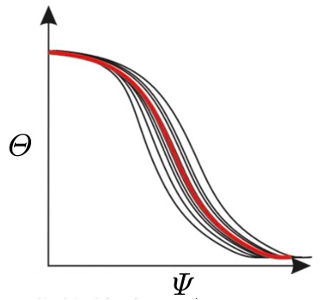
\includegraphics{Figures/尺度转换/土壤水力参数尺度转换示意图.png}
\caption[土壤水力参数尺度转换示意图]{土壤水力参数尺度转换示意图。其中黑线表示一个模式模拟单元(patch)内所有细网格对应的土壤水分特征曲线,而红线代表该patch内到达所有细网格土壤水力特征曲线距离最短的特征曲线,该曲线对应的参数即作为patch尺度上的特征参数}
\label{fig:土壤水力参数尺度转换示意图}
\end{figure}
}

以升尺度~\citet{campbell1974} 模型中的参数为例,具体方法如下:首先,给出patch内所有细网格对应的土壤水分特征曲线和土壤导水率曲线关系,即通过每个细网格中的参数$\psi_{si}$、$\lambda_{i}$、$\theta_{si}$和$K_{si}$,计算下列由24个特征土壤水势组成的土壤水势向量对应的土壤含水量向量$\theta_i=\theta_{si}\left(\frac{\psi}{\psi_{si}}\right)^{-\frac{1}{B_{i}}}$和土壤导水率向量$K_i=K_{si}\left(\frac{\psi}{\psi_{si}}\right)^{-\frac{3}{B_{i}}-2}$:
\begin{equation}
\begin{aligned}
\psi&=[-1,-5,-10,-20,-30,-40,-50,-60,-70,-90,-110,-130,-150,-170,\\
&-210,-300,-345  -690,-1020,-5100,-15300,-20000,-100000,-1000000]
\end{aligned}
\end{equation}
其次,在patch中求解所有细网格饱和土壤含水量$\theta_{si}$的面积加权平均值作为patch尺度下的饱和土壤含水量$\theta_s$。最后,在patch中求解下列极值问题,得到patch尺度下的参数$\hat{\psi}_{s}$、$\hat{B}$和$\hat{K_s}$:
\begin{equation}
\chi\left(\hat{\psi_s}, \hat{B}, \hat{K_s}\right)=\min\left\{ \sum_{j=1}^{24}\sum_{i=1}^{N}\left[\left(\frac{\hat{\theta}\left(\psi_j\right)-\theta_i\left(\psi_j\right)}{\theta_s}\right)^2
+\left(\frac{\log_{10}\hat{K}\left(\psi_j\right)-\log_{10}K_i\left(\psi_j\right)}{\log_{10}K_s}\right)^2\right]\right\}
\end{equation}
其中$N$表示每个patch中细网格的数量;$\theta_s$和$K_s$分别表示patch尺度下的土壤饱和含水量和土壤饱和导水率,用以在求解上述极值问题中对土壤水力特征曲线关系和土壤导水率曲线关系进行标准化;$\hat{\theta}$和$\hat{K}$分别表示在patch尺度下针对每个土壤水势待确定的实际土壤含水量和土壤导水率。上述问题最终解出的使$\hat{\theta}$和$\hat{K}$满足最小值问题对应的参数$\hat{\psi}_{s}$、$\hat{B}$和$\hat{K_s}$即作为每个patch的土壤水力特征曲线和土壤导水率曲线对应的参数,是使得每个patch的特征曲线最为接近其所包含的全部细网格特征曲线的最优参数。求解极值问题所使用的数值算法为优化后的Levenberg-Marquard非线性最小二乘算法~\citep{Montzka2017scale}。patch中的~\citet{van1980closed}--\citet{mualem1976new}土壤水力特征曲线参数和土壤导水率曲线参数亦可通过上述升尺度方法类似得到。

此方法的最大优势为升尺度后的参数仍可保持土壤水力特征曲线和土壤导水率曲线关系,并且与所有细网格具有最大程度上的物理一致性。